\subsubsection{Collision Detection}
\noindent {\em Auteur: Jef Versyck}
\\\\
Aangezien polyhedra geen mooie cirkels kunnen zijn, moet de collision detection veranderd worden. Eerst wordt er vergeleken of de afstand tussen de twee centra van de objecten (een polyhedron en de drone) kleiner is dan beide hun radii opgeteld. De radius van een polyhedron wordt gedefiniëerd als de grootste afstand tussen het centrum van de polyhedra en zijn punten. \\
\noindent
Vervolgens wordt er getest of de loodrechte afstand op het vlak van een Triangle vanuit het middelpunt van de drone kleiner is dan de straal van de drone. Hierbij wordt het vlak waarin de Triangle zich bevindt, berekend aan de hand van het kruisproduct van twee vectoren van de Triangle en een hoekpunt ervan. Vervolgens wordt de loodrechte projectie op het vlak bepaald. Dit punt heet P. In formulevorm: 
\begin{gather*}
	a*x + b*y + c*z = d \\ 
	t = -\frac{a * x_{drone} + b * y_{drone} + c * z_{drone} - d}{a^2 + b^2 + c^2}  \\ P =
	\begin{Bmatrix}
	a*t + x_{drone}\\ 
	b*t + y_{drone}\\ 
	c*t + z_{drone}
	\end{Bmatrix}
\end{gather*}

\noindent
 Dit is echter niet genoeg. De loodrechte projectie van het massacentrum  kan zich buiten de Triangle bevinden en zo een foutief resultaat geven. Om te zien of het punt zich binnen de Triangle bevindt, wordt aan de hand van barycentrische coördinaten gecontroleerd. Het principe hierachter is dat elk punt P in de driehoek geschreven kan worden als een lineaire combinatie van de hoekpunten (A, B en C) van een driehoek. De som van alle coëfficiënten moet gelijk zijn aan 1 en alle coëfficiënten moeten groter zijn dan 0. In formulevorm:
 
 \begin{gather*}
 	P = u*A + v*B + w*C \\
 	0 \le u,v,w \le 1 \\
 	u + v + w = 1
 \end{gather*}

%TODO https://www.scratchapixel.com/lessons/3d-basic-rendering/ray-tracing-rendering-a-triangle/barycentric-coordinates hierbij als referentie zetten

\noindent
Dit lost echter niet alle problemen op. De drone kan de polyhedron raken, maar de loodrechte afstand kan buiten de triangle liggen. Hiervoor werd ten tijde van schrijven nog geen oplossing gevonden. Zie figuur \ref{fig:CollisionDetectionProbleem} voor verduidelijking. Het snijpunt ligt duidelijk buiten de Triangle, maar toch snijdt de drone de Triangle.
\begin{figure}[h]
	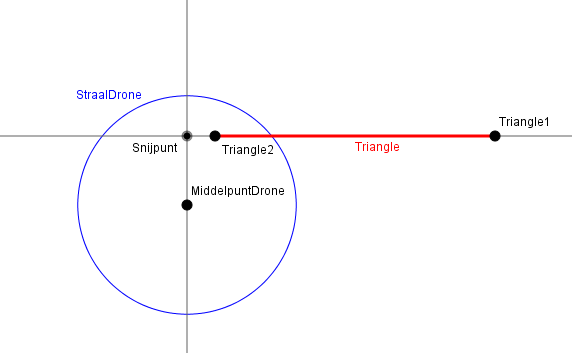
\includegraphics[width=1\textwidth]{CollisionDetectionProbleem.png}
	\caption{Een voorbeeld van het probleem met de huidige collision detection.\\ }
	\label{fig:CollisionDetectionProbleem}
\end{figure}